\documentclass{article}
\usepackage[T1]{fontenc}
\usepackage{lmodern}
\usepackage{graphicx}
\usepackage{amsmath,amssymb}
\usepackage[a4paper,margin=2cm]{geometry}
\usepackage[absolute,overlay]{textpos}
\setlength{\TPHorizModule}{1mm}
\setlength{\TPVertModule}{1mm}
\usepackage[indonesian]{babel}
\usepackage{hyperref}
\setlength{\emergencystretch}{2em}
% unit: Halaman 18

\begin{document}

% === Halaman 18 (llm) ===

\section*{Transformasi $SubBytes()$}

\vspace{202.26mm}

\begin{itemize}
    \item $SubBytes()$ melakukan operasi substitusi dengan memetakan setiap byte dari array state dengan menggunakan S-box.
\end{itemize}

\vspace{10mm}

% deskripsi: Tabel S-box yang digunakan dalam transformasi SubBytes pada algoritma AES, berisi pemetaan nilai heksadesimal dari indeks baris dan kolom ke nilai substitusinya.
% bbox normalisasi: [0.2060, 0.2700, 0.7380, 0.9510]
\begin{textblock*}{111.72mm}(43.26mm,80.19mm)
\noindent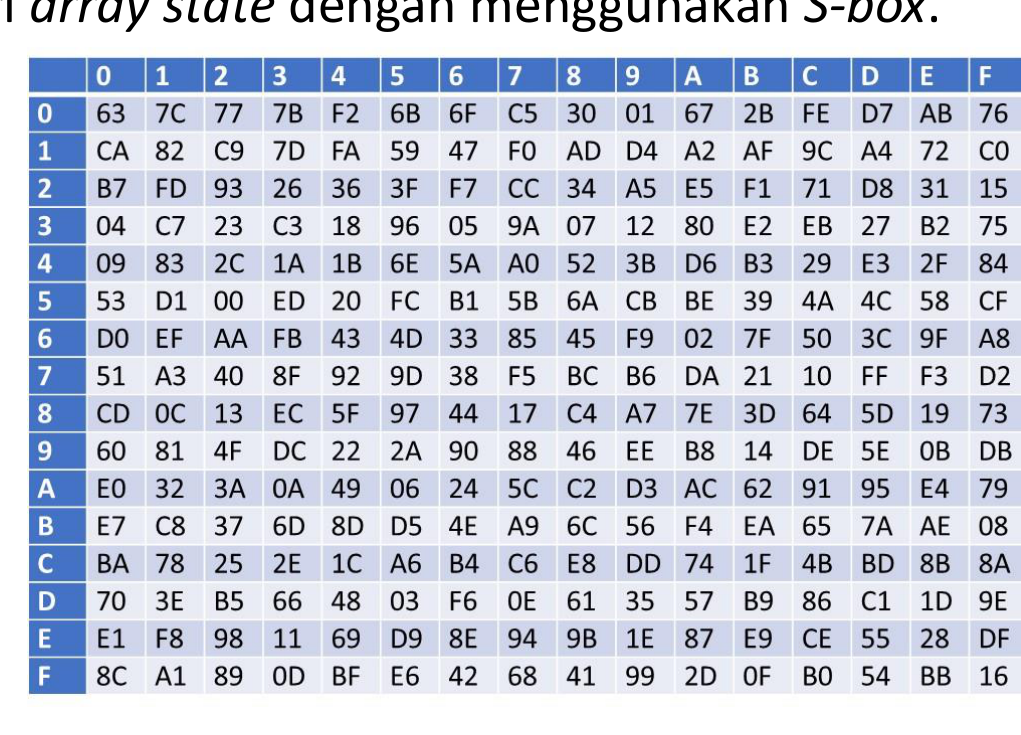
\includegraphics[width=111.72mm,height=202.26mm]{../../images/llm/page_018_img_01.png}%
\end{textblock*}

\end{document}
